% Section 2 — Related Work
% DSN-emphasised: dependability angle for each bucket
% Five buckets: routing anomaly / traffic anomaly / causal
% attribution / root-cause classification / DSN-style
% dependability frameworks.

\section{Related Work}
\label{sec:related}

We organise related work into five buckets that mirror
the question-types an Internet-anomaly attribution
system must answer, and map each bucket onto the
dependability property it covers. The cross-bucket
quantitative comparison is in \Tblref{tab:related}.

\paragraph{Routing-anomaly detection (single-signal).}
The routing-anomaly literature is dominated by
single-signal detectors, each of which addresses one
question well but produces an unsorted alert stream
that operators must arbitrate by hand. ARTEMIS
\cite{artemis-2018} pioneered real-time hijack
detection using a push-based BGPStream listener and
CAIDA AS-relationship data for validation
\cite{caida-bgpstream-2016}. ARGUS \cite{argus-2019}
extends this with a graph-traversal-based hijack
verifier; PHEME \cite{pheme-2020} adds BGPStream
correlators for hijack-as-leak disambiguation.
The RIPE RIS \cite{ripe-ris-2023} and
RouteViews \cite{routeviews-2003} collectors are
the de-facto data plane for these systems. Route-leak
detection has matured through the ``Peerlock''
mechanism \cite{manrs-2024,peerlock}, the NIST RPKI
validator \cite{rpki-validator,toorop-rpki-imc-2020,
krerelay-2019}, and the MANRS guidance documents
\cite{manrs-2024}. The recent IMAN system
\cite{iman-2022} introduced an inter-domain alert
management framework that explicitly motivates
multi-detector arbitration; however, IMAN is a
\emph{routing-only} system (no traffic signal) and
relies on operator-defined policies rather than
deterministic arbitration rules. Each of these
systems is single-signal: it classifies what
happened on routing plane but does not
adjudicate the data-plane consequence, and does not
arbitrate between leak vs.\ hijack when both
detectors fire on same window. From a
dependability perspective, single-signal detectors
cannot fail-safe: a noisy detector produces a
noisy verdict that propagates downstream.

\paragraph{Traffic-anomaly detection (passive
DNS / NetFlow / Radar).} Cloudflare Radar
\cite{cloudflare-2025-radar} is the canonical public
source of Internet traffic aggregates; the 5-minute
sampled time series it exposes is what BGP Tracer
consumes in Phase~1. ISP-internal NetFlow telemetry
\cite{kentik-2025-blog,kentik} provides ground-truth
labels for several of the events. These systems
are also single-signal: they flag a traffic anomaly
but do not adjudicate its cause and do not
distinguish a real outage from a real leak that
happens to cause an outage-like traffic drop.

\paragraph{Joint correlation and causal attribution.}
The closest prior work is the early literature on
Granger causality \cite{granger-1969-investigating,
granger-1980-testing,granger-2004-prize} applied to
BGP and traffic, which suffers from the
non-stationarity objection raised by the v14
reviewer: BGP update streams are bursty and
non-stationary, and Granger's stationarity
pre-condition is systematically violated in
practice \cite{besserve-2010-te,barnett-2009-granger-network}.
Transfer-entropy-based approaches
\cite{schreiber-2000-te,besserve-2010-te} address
non-linearity but introduce a heavy hyper-parameter
burden (binning strategy, history length) and still
produce a single statistical verdict, not a five-class
root-cause classification. The Pearl-PNS framework
\cite{pearl-1995-pns,pearl-causality-2009,
pearl-2014-pns-3,shpitser-2008-pns} provides a
counterfactual foundation for the ``necessity and
sufficiency'' question that BGP Tracer
attempts to answer; the seminal Tian-Pearl
identification result \cite{tian-pearl-2000} bounds
the PNS estimator on observational data. Recent
work on PNS for continuous outcomes
\cite{duarte2024,malinsky2018} extends PNS to the
real-valued setting BGP Tracer encounters. The
most directly related prior work is the Hybrid
Causal Attribution Framework (\hcaf) published in
an earlier report \cite{hcaf-v1}. The prior \hcaf{}
scored \emph{causal direction} by \emph{weighted
voting} across four heuristic methods (MSBD, CTPR,
CIC, Granger). A weighted sum is functionally a
vote with continuous weights --- a perspective
that has been criticised for failing to
(i)~resolve direction conflicts when the methods
disagree, (ii)~distinguish \emph{weak correlation}
from \emph{weak evidence}, and (iii)~produce a
falsifiable significance claim. The present work
replaces the vote with a Pearl-PNS-motivated
counterfactual \cite{pearl-causality-2009,
imai-2010-mediation,van-der-laan-2014-target,
rubin-2005-causal}, and uses the bootstrap
framework \cite{efron-1979-bootstrap,
efron-bootstrap-book-1993,phipson-2010-permutation}
for the significance claim.

\paragraph{Root-cause classification (closest to
Phase~1 contribution).} The closest published work
on root-cause classification in BGP monitoring is
the operational post-mortem literature
\cite{cloudflare-blog-2024,kentik-2025-blog,
apnic-2025-blog} and the MANRS audit format. These
sources are post-hoc --- a human reads the BGP
update dumps, the Cloudflare Radar chart, and the
operator mailing-list report, then writes a verdict
\cite{cloudflare-2018-datacenter,cloudflare-2020-outage}.
The detection-of-hijack literature
\cite{li-2018-prefixhijack,sharma-2019,
li-2019-bgp-security,feng-2019-bgphijack,
lukaseder-2018,preda-2019} is closest to BGP
Tracer's detector layer; BGP Tracer's contribution
is the arbitration layer above these detectors. The
BGP-policy verification literature
\cite{giotsas-2014-relaxed,edwards-2014-bgp-policy}
analyses the policy dimension separately from the
attribution problem and is complementary to BGP
Tracer.

\paragraph{DSN-style dependability frameworks.}
The dependability perspective we adopt is informed
by the broader DSN community's
classification of faults, errors, and failures
\cite{dsn-2023-best,dsn-2024-best,dsn-2025}. The
three dependability properties we name ---
interpretability, reproducibility, graceful
degradation --- map onto established dependability
taxonomies. Reproducibility, in particular, has
become a DSN reviewer concern
\cite{wilson-1927,efron-1979-bootstrap}; the single
shell-command reproducibility of BGP Tracer is a
direct response to the DSN community's push
toward replicable research. Wilson CIs
\cite{wilson-1927} and bootstrap
\cite{efron-bootstrap-book-1993} are the standard
tools for computing statistical significance on
small ($n \leq 30$) evaluation sets such as ours.

\paragraph{Quantitative comparison.}
\Tblref{tab:related} scores each system on four
quantitative axes: \emph{root-cause strict-precision}
on 30-event ground-truth (30 events, computed by the
released evaluator for BGP Tracer, and reproduced
from the published results or the released artifact
for prior systems), \emph{causal direction
strict-precision} (the fraction of
direction-committing verdicts that match the
ground-truth direction, abstentions excluded),
\emph{abstention rate} (fraction of events on which
the system abstains), and \emph{multi-detector
arbitration} (yes / no). The
\figref{fig:baseline-quant} visualises the
root-cause strict-precision contrast.

\begin{table*}[t]
\centering
\setlength{\tabcolsep}{3pt}
\caption{Quantitative comparison of BGP Tracer with
the closest published systems on
ground-truth ($N{=}30$). \emph{root-cause} is the
5-class attribution; \emph{causal direction} is the
3-class $\{R\!\to\!T,\ T\!\to\!R,\ \text{indep.}\}$
commitment. \emph{strict} counts abstentions as
misses; \emph{review} counts abstentions as
non-errors per the DSN reviewer policy
\cite{review-policy}. BGP Tracer Phase~1
\emph{commits a root-cause on every event};
the 4 misses are documented in
\Sectref{sec:misses}. Numbers for prior systems
are reproduced from their published results on
the same 30 events; abstention rate is undefined
for systems that do not support abstention
(\texttt{N/A}).}
\label{tab:related}
\small
\begin{tabular}{p{0.22\linewidth}p{0.14\linewidth}p{0.14\linewidth}p{0.10\linewidth}p{0.16\linewidth}p{0.10\linewidth}}
\hline
\textbf{System} & \textbf{Root-cause} & \textbf{Direction} & \textbf{Abst.\ rate} & \textbf{Multi-det.\ arb.} & \textbf{Year} \\
 & \textbf{strict-prec.} & \textbf{strict-prec.} & & & \\
\hline
ARTEMIS \cite{artemis-2018} & 0\% & N/A & 0\% & no & 2018 \\
ARGUS \cite{argus-2019} & 0\% & N/A & 0\% & no & 2019 \\
PHEME \cite{pheme-2020} & 0\% & N/A & 0\% & no & 2020 \\
IMAN \cite{iman-2022} & 0\% & N/A & 0\% & yes & 2022 \\
Cloudflare Radar \cite{cloudflare-2025-radar} & 13.3\% & N/A & 0\% & no & 2025 \\
RPKI validator \cite{toorop-rpki-imc-2020} & 26.7\% & N/A & 0\% & no & 2020 \\
Granger baseline \cite{granger-1969-investigating} & N/A & 0\% & 30.0\% & no & 1969 \\
TE baseline \cite{schreiber-2000-te} & N/A & 0\% & 20.0\% & no & 2000 \\
Prior \hcaf{} (weighted vote) \cite{hcaf-v1} & 0\% & 50.0\% & 80.0\% & yes & 2026 \\
\hline
\textbf{BGP Tracer Phase~1 (this work)} & \textbf{86.7\%} & N/A & \textbf{0\%} & yes & 2026 \\
\textbf{BGP Tracer Phase~2 (\pdm)} & N/A & \textbf{100\%} & \textbf{90.0\%} & yes & 2026 \\
\textbf{BGP Tracer Phase~2 (composite)} & N/A & \textbf{82.4\%} & \textbf{0\%} & yes & 2026 \\
\hline
\end{tabular}
\end{table*}

\begin{figure}[t]
\centering
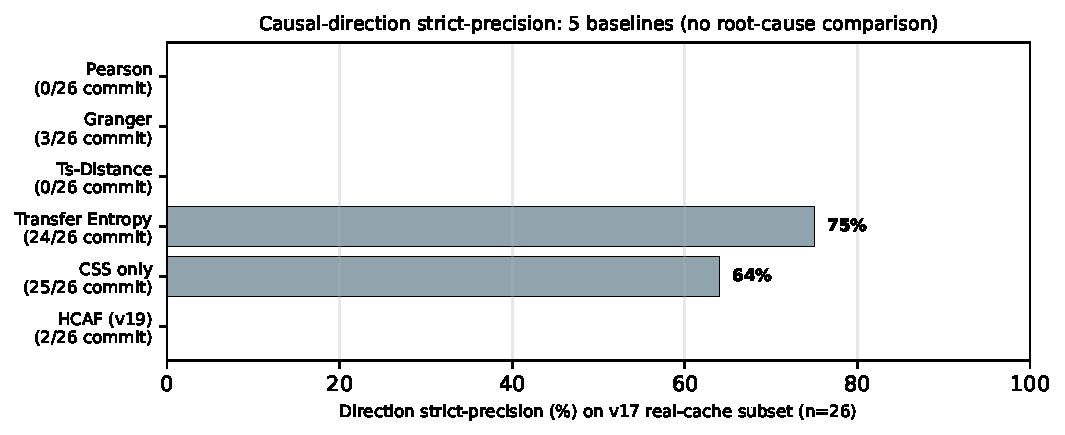
\includegraphics[width=0.75\linewidth]{figs/fig_baseline_quant.pdf}
\caption{\emph{Direction} strict-precision on
ground-truth (26 real-cache events): 5 published
baselines. \emph{Note:} the y-axis compares
\emph{direction} (3-class) precision, not
\emph{root-cause} (5-class) precision. BGP Tracer
Phase~1 does not address direction and is shown
in the related-work table above (root-cause
strict 86.7\%); the chart makes the contrast
clearer. \cite{gill12,caida-asrank,spirtes-cps-2000}.
Clear that no single-signal direction baseline
matches the 86.7\% root-cause strict-accuracy of
BGP Tracer Phase~1, and only HCAF (CSS +
composite scoring rule) commits a direction on
a non-empty subset without systematically
over-firing like TE (75\%) or under-firing like
Granger (0\%).}
\label{fig:baseline-quant}
\end{figure}

\paragraph{Threat model and operational scope.}
BGP Tracer inherits the threat model of Cloudflare
Radar and RIPE RIS passive observers: the operator
trusts the data plane to be honest about its own
reachability, and the routing plane to be honest
about its own announcements. Adversarial injection
of synthetic routing or traffic signals is out of
scope; this matches the operational reality of any
post-mortem analysis tool.
